\section{Wireless Characteristics}
\label{sec:wirelesscharacteristics}


% \begin{figure*}
% \begin{minipage}{0.3\textwidth}
% \includegraphics[width=1\textwidth]{Figs4Paper/GaussianDistr/gaussian.eps}
% \caption{The distribution of RSS observed on a sniffer}
% \label{fig:distribution}
% \end{minipage}\quad %
% \begin{minipage}{0.3\textwidth}%
% \includegraphics[width=1\textwidth]{Figs4Paper/TxPower/Tx_PowerLevels.eps}
% \caption{RSS as a function of the Tx-power of a device.}
% \label{fig:txpower}
% \end{minipage}\quad%
% \begin{minipage}{0.3\textwidth}%
% 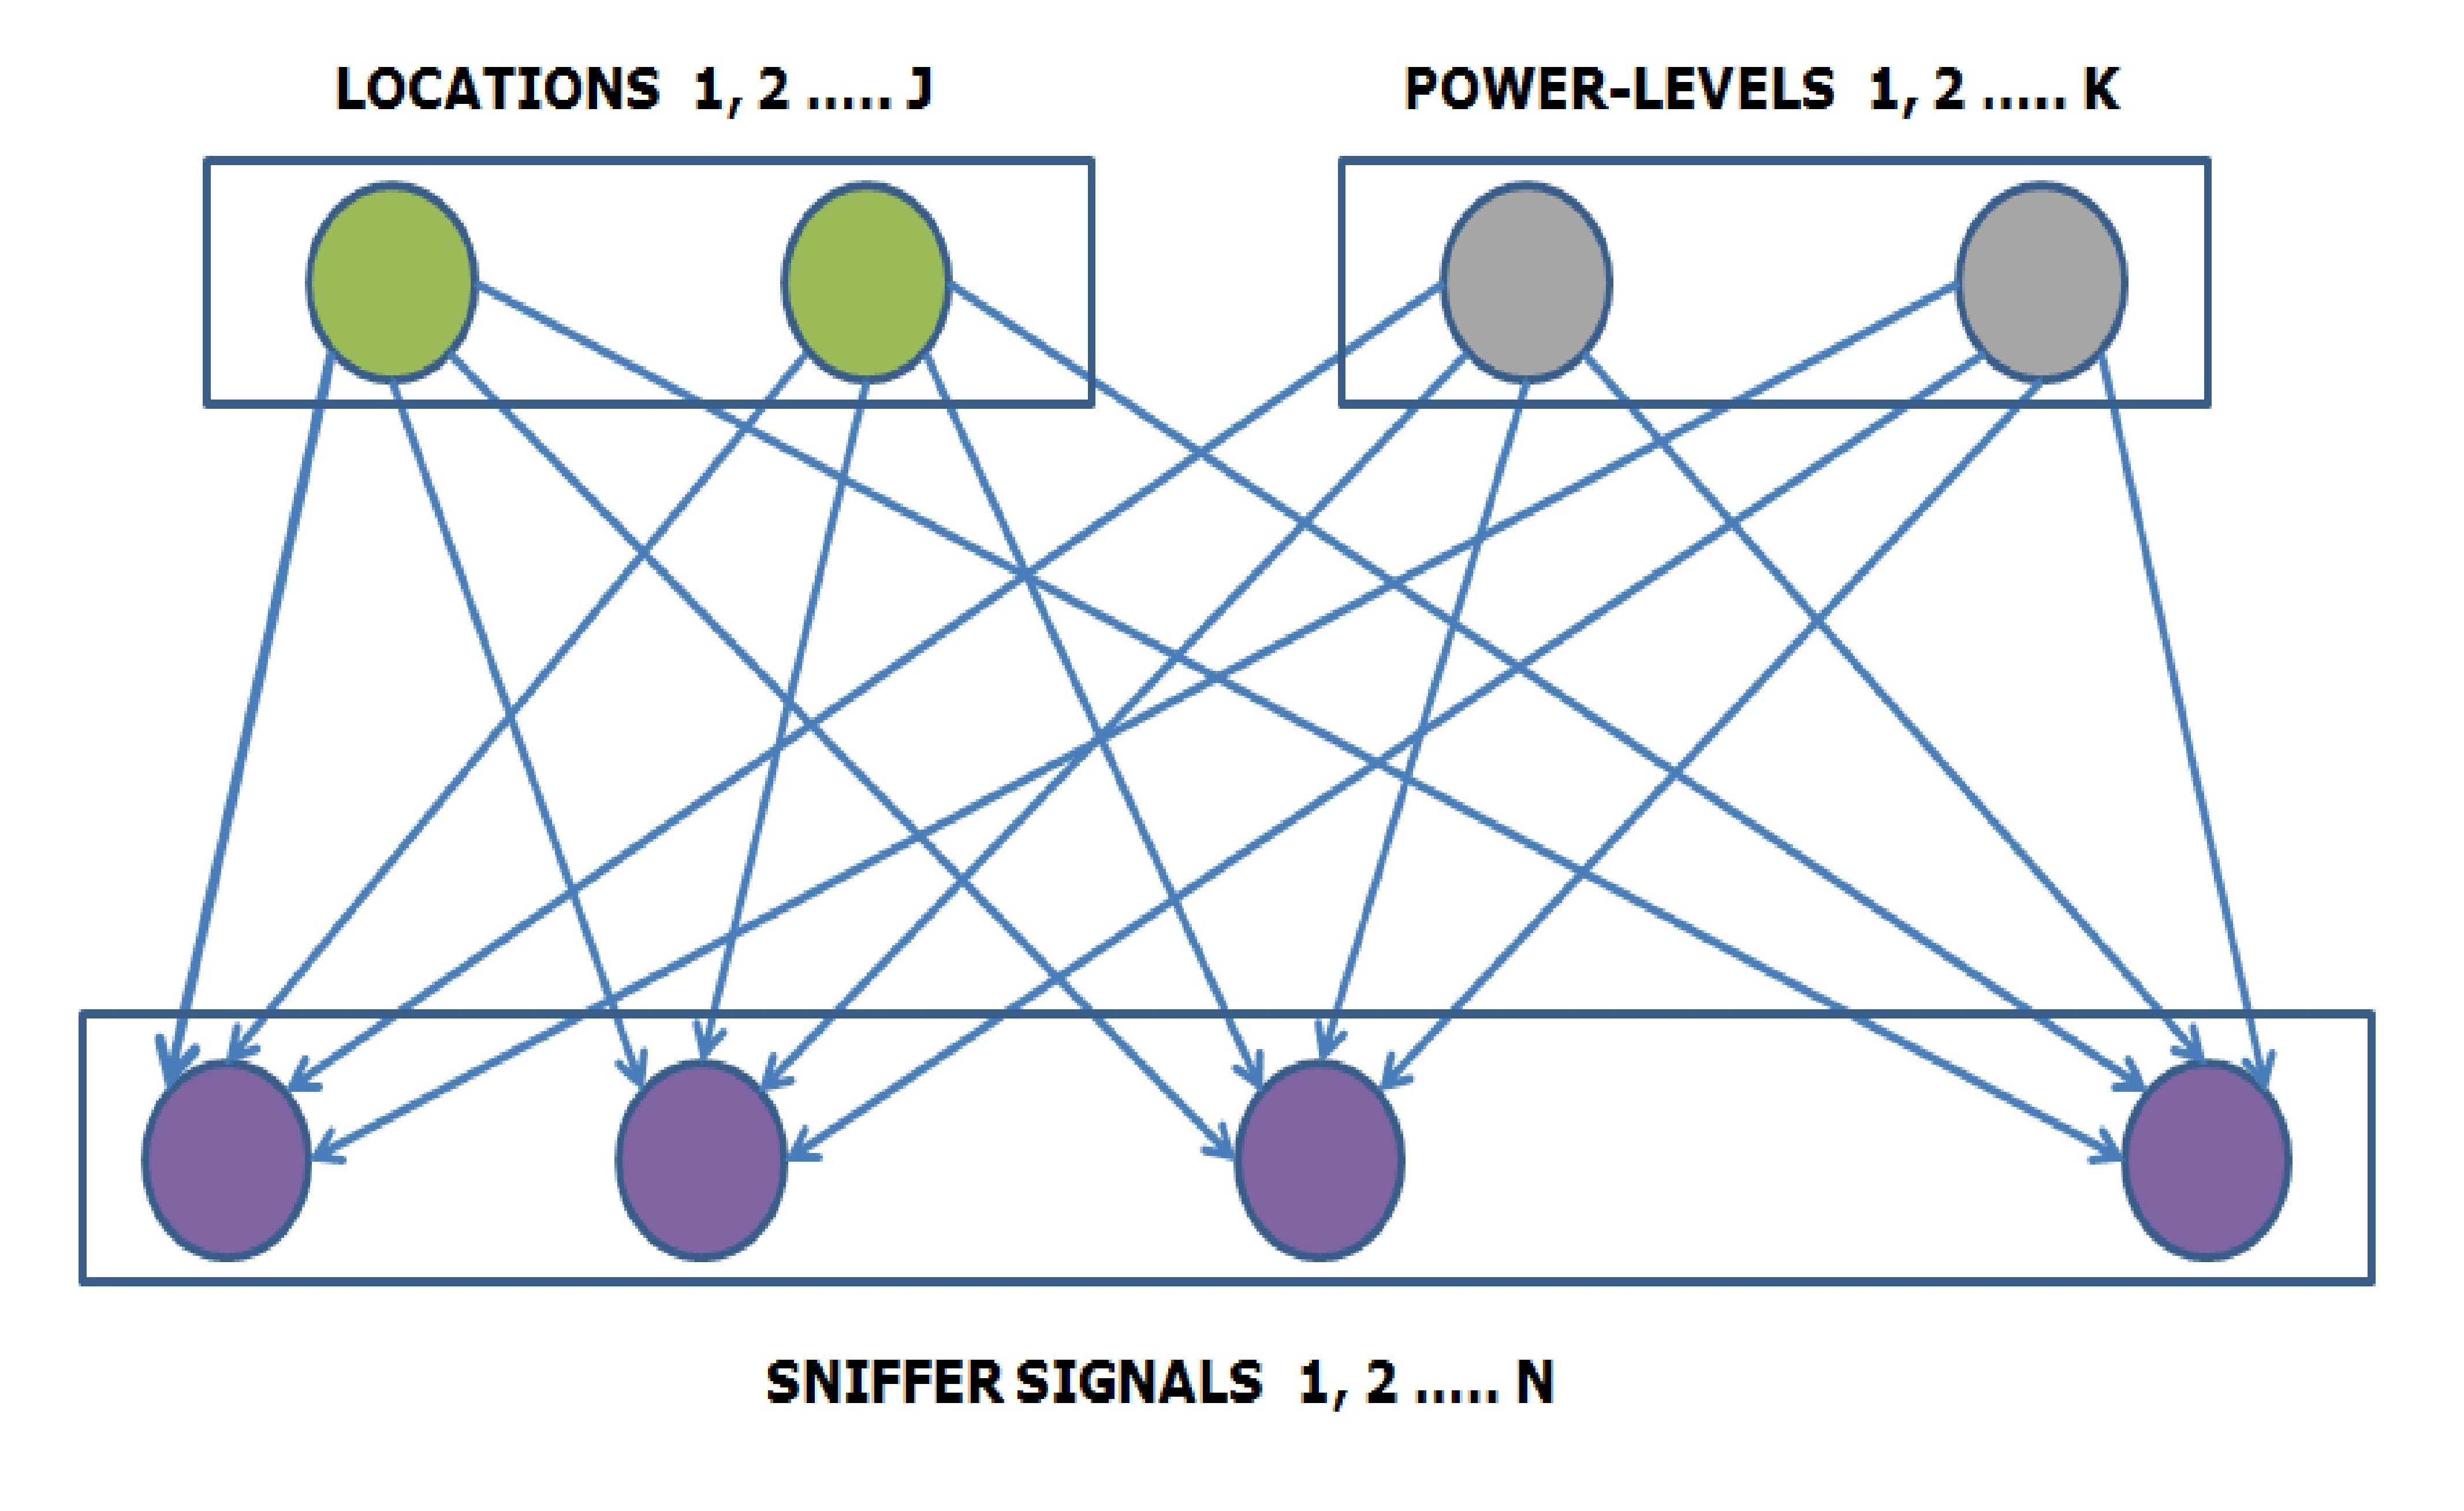
\includegraphics[width=1\textwidth]{Figs4Paper/gmm.eps}
% \caption{The GMM for our problem}
% \label{fig:gmm}
% \end{minipage}%
% \end{figure*}


% \begin{figure*}[h!]
% \begin{minipage}{0.52\textwidth}
% %\subfloat[big]{\label{subfig:a}\includegraphics[width=1\textwidth]{Figs/gaussian.eps}} \\%
% %\subfloat[big2]{\label{subfig:a}\includegraphics[width=1\textwidth]{Figs/gaussian.eps}}%
% 
% \includegraphics[width=1\textwidth]{Figs/gaussian.eps}
% \caption{first minipage}
% \end{minipage}\quad %
% \begin{minipage}{0.33\textwidth}%
% \subfloat[small]{\label{subfig:b}\includegraphics[width=1\textwidth]{Figs/gaussian.eps}}\\%
% \subfloat[small]{\label{subfig:c}\includegraphics[width=1\textwidth]{Figs/gaussian.eps}}%
% \caption{second minipage}
% \end{minipage}%


 %\label{fig:diamond_lattice}
 %\caption{Face-Center-Cubic - \ref{subfig:a}  \ref{subfig:b} \ref{subfig:c} }

%\end{figure*}



% \begin{figure}[h!]
%   \centering
%     \epsfig{file=Figs/gaussian.eps, height=1.5in, width=2.5in}
%   \caption{ Received Signal Strength at a sniffer from a laptop operating at a fixed power-level }
%   \label{fig:gaussian}
% \end{figure}
% 
% \begin{figure}[h!]
% \centering
%   \epsfig{file=Figs/Tx_PowerLevels.eps, height=1.5in, width=2.5in}
%   \caption{Signal strength readings from three different receivers of a signal from a signal transmitter, with the transmitter varying it Tx-Power}
%   \label{fig:txpower}
% \end{figure}

Our system is based on the 802.11 wireless networking protocol, which is
inexpensive and widely deployed in enterprise offices and academic
campuses. 802.11 uses 11 channels in the ISM band. Signal
propagation in this band is complex and in this section, we identify the different
causes of variation in the wireless channel quality and how we factor
them into our model. Our approach is server-based, where we capture
client packets using sniffers. As such, we are mainly concerned with the
variations that affect the Received Signal Strength (RSS) on the
sniffer. In this section, experimentally validate two observations that have been made previously
in wireless-localization literature. We model our problem around these
two observations. 

\subsection{Distribution of Signal Strength}
\label{subsec:distributionofsignalstrength}

\begin{figure} [h!]
\centering
\epsfig{file=Figs4Paper/GaussianDistr/gaussian.eps, height=1.5in, width=2.5in}
\caption{The distribution of RSS observed on a sniffer}
\label{fig:distribution}
\end{figure}


Figure \ref{fig:distribution} shows the distribution of Received Signal
Strength values observed by a sniffer located a fixed distance apart
from a transmitting client. The Tx-client is a Dell laptop having a
Ubiquiti XR2 wireless card and is using a fixed power-level for wireless
transmissions. 

We observe that the Signal Strength distribution is roughly Gaussian. In
\cite{Tao:2003:WLL:941311.941314} Tao et al also make similar observations.
\cite{Haeberlen:2004:PRL:1023720.1023728, Moraes:2006:CWL:1164783.1164799} etc also model signal intensity
as a normal distribution.

\subsection{Transmission Power}
\label{subsec:transmissionpower}

\begin{figure} [h!]
\centering
\epsfig{file=Figs4Paper/TxPower/Tx_PowerLevels.eps, height=1.5in, width=2.5in}
\caption{RSS as a function of the Tx-power of a device.}
\label{fig:txpower}
\end{figure}

Figure \ref{fig:txpower} shows how the observed signal strength changes
as the transmission power is varied. Our experiments validate the
observations made in \cite{Tao:2003:WLL:941311.941314} by Tao et al in that the observed
signal strength is linearly proportional to the transmission power.
